% Options for packages loaded elsewhere
\PassOptionsToPackage{unicode}{hyperref}
\PassOptionsToPackage{hyphens}{url}
%
\documentclass[
]{article}
\usepackage{amsmath,amssymb}
\usepackage{iftex}
\ifPDFTeX
  \usepackage[T1]{fontenc}
  \usepackage[utf8]{inputenc}
  \usepackage{textcomp} % provide euro and other symbols
\else % if luatex or xetex
  \usepackage{unicode-math} % this also loads fontspec
  \defaultfontfeatures{Scale=MatchLowercase}
  \defaultfontfeatures[\rmfamily]{Ligatures=TeX,Scale=1}
\fi
\usepackage{lmodern}
\ifPDFTeX\else
  % xetex/luatex font selection
\fi
% Use upquote if available, for straight quotes in verbatim environments
\IfFileExists{upquote.sty}{\usepackage{upquote}}{}
\IfFileExists{microtype.sty}{% use microtype if available
  \usepackage[]{microtype}
  \UseMicrotypeSet[protrusion]{basicmath} % disable protrusion for tt fonts
}{}
\makeatletter
\@ifundefined{KOMAClassName}{% if non-KOMA class
  \IfFileExists{parskip.sty}{%
    \usepackage{parskip}
  }{% else
    \setlength{\parindent}{0pt}
    \setlength{\parskip}{6pt plus 2pt minus 1pt}}
}{% if KOMA class
  \KOMAoptions{parskip=half}}
\makeatother
\usepackage{xcolor}
\usepackage[margin=1in]{geometry}
\usepackage{color}
\usepackage{fancyvrb}
\newcommand{\VerbBar}{|}
\newcommand{\VERB}{\Verb[commandchars=\\\{\}]}
\DefineVerbatimEnvironment{Highlighting}{Verbatim}{commandchars=\\\{\}}
% Add ',fontsize=\small' for more characters per line
\usepackage{framed}
\definecolor{shadecolor}{RGB}{248,248,248}
\newenvironment{Shaded}{\begin{snugshade}}{\end{snugshade}}
\newcommand{\AlertTok}[1]{\textcolor[rgb]{0.94,0.16,0.16}{#1}}
\newcommand{\AnnotationTok}[1]{\textcolor[rgb]{0.56,0.35,0.01}{\textbf{\textit{#1}}}}
\newcommand{\AttributeTok}[1]{\textcolor[rgb]{0.13,0.29,0.53}{#1}}
\newcommand{\BaseNTok}[1]{\textcolor[rgb]{0.00,0.00,0.81}{#1}}
\newcommand{\BuiltInTok}[1]{#1}
\newcommand{\CharTok}[1]{\textcolor[rgb]{0.31,0.60,0.02}{#1}}
\newcommand{\CommentTok}[1]{\textcolor[rgb]{0.56,0.35,0.01}{\textit{#1}}}
\newcommand{\CommentVarTok}[1]{\textcolor[rgb]{0.56,0.35,0.01}{\textbf{\textit{#1}}}}
\newcommand{\ConstantTok}[1]{\textcolor[rgb]{0.56,0.35,0.01}{#1}}
\newcommand{\ControlFlowTok}[1]{\textcolor[rgb]{0.13,0.29,0.53}{\textbf{#1}}}
\newcommand{\DataTypeTok}[1]{\textcolor[rgb]{0.13,0.29,0.53}{#1}}
\newcommand{\DecValTok}[1]{\textcolor[rgb]{0.00,0.00,0.81}{#1}}
\newcommand{\DocumentationTok}[1]{\textcolor[rgb]{0.56,0.35,0.01}{\textbf{\textit{#1}}}}
\newcommand{\ErrorTok}[1]{\textcolor[rgb]{0.64,0.00,0.00}{\textbf{#1}}}
\newcommand{\ExtensionTok}[1]{#1}
\newcommand{\FloatTok}[1]{\textcolor[rgb]{0.00,0.00,0.81}{#1}}
\newcommand{\FunctionTok}[1]{\textcolor[rgb]{0.13,0.29,0.53}{\textbf{#1}}}
\newcommand{\ImportTok}[1]{#1}
\newcommand{\InformationTok}[1]{\textcolor[rgb]{0.56,0.35,0.01}{\textbf{\textit{#1}}}}
\newcommand{\KeywordTok}[1]{\textcolor[rgb]{0.13,0.29,0.53}{\textbf{#1}}}
\newcommand{\NormalTok}[1]{#1}
\newcommand{\OperatorTok}[1]{\textcolor[rgb]{0.81,0.36,0.00}{\textbf{#1}}}
\newcommand{\OtherTok}[1]{\textcolor[rgb]{0.56,0.35,0.01}{#1}}
\newcommand{\PreprocessorTok}[1]{\textcolor[rgb]{0.56,0.35,0.01}{\textit{#1}}}
\newcommand{\RegionMarkerTok}[1]{#1}
\newcommand{\SpecialCharTok}[1]{\textcolor[rgb]{0.81,0.36,0.00}{\textbf{#1}}}
\newcommand{\SpecialStringTok}[1]{\textcolor[rgb]{0.31,0.60,0.02}{#1}}
\newcommand{\StringTok}[1]{\textcolor[rgb]{0.31,0.60,0.02}{#1}}
\newcommand{\VariableTok}[1]{\textcolor[rgb]{0.00,0.00,0.00}{#1}}
\newcommand{\VerbatimStringTok}[1]{\textcolor[rgb]{0.31,0.60,0.02}{#1}}
\newcommand{\WarningTok}[1]{\textcolor[rgb]{0.56,0.35,0.01}{\textbf{\textit{#1}}}}
\usepackage{graphicx}
\makeatletter
\def\maxwidth{\ifdim\Gin@nat@width>\linewidth\linewidth\else\Gin@nat@width\fi}
\def\maxheight{\ifdim\Gin@nat@height>\textheight\textheight\else\Gin@nat@height\fi}
\makeatother
% Scale images if necessary, so that they will not overflow the page
% margins by default, and it is still possible to overwrite the defaults
% using explicit options in \includegraphics[width, height, ...]{}
\setkeys{Gin}{width=\maxwidth,height=\maxheight,keepaspectratio}
% Set default figure placement to htbp
\makeatletter
\def\fps@figure{htbp}
\makeatother
\setlength{\emergencystretch}{3em} % prevent overfull lines
\providecommand{\tightlist}{%
  \setlength{\itemsep}{0pt}\setlength{\parskip}{0pt}}
\setcounter{secnumdepth}{-\maxdimen} % remove section numbering
\ifLuaTeX
  \usepackage{selnolig}  % disable illegal ligatures
\fi
\usepackage{bookmark}
\IfFileExists{xurl.sty}{\usepackage{xurl}}{} % add URL line breaks if available
\urlstyle{same}
\hypersetup{
  hidelinks,
  pdfcreator={LaTeX via pandoc}}

\author{}
\date{\vspace{-2.5em}}

\begin{document}

\newpage

\section{Exercice 6}\label{exercice-6}

Les données pour cet exercice sont stockées dans le fichier
\texttt{RM04data.csv}. Commençons par charger ces données. Nous ne
prennons que les lignes 5 et 6.

\begin{Shaded}
\begin{Highlighting}[]
\CommentTok{\# La fonction read\_csv2 est issue du package readr qui permet des imports}
\CommentTok{\# exports facilités dans R}
\NormalTok{df }\OtherTok{\textless{}{-}} \FunctionTok{read.csv}\NormalTok{(}\StringTok{"../data/RM04data.csv"}\NormalTok{, }\AttributeTok{sep =} \StringTok{\textquotesingle{},\textquotesingle{}}\NormalTok{, }\AttributeTok{header =} \ConstantTok{FALSE}\NormalTok{)}
\NormalTok{df }\OtherTok{\textless{}{-}}\NormalTok{ df[}\DecValTok{5}\SpecialCharTok{:}\DecValTok{6}\NormalTok{,]}

\NormalTok{columns\_names }\OtherTok{=} \FunctionTok{c}\NormalTok{(}\StringTok{"xi"}\NormalTok{,}\StringTok{"ui"}\NormalTok{)}
\NormalTok{observations\_labels }\OtherTok{\textless{}{-}} \FunctionTok{paste}\NormalTok{(}\StringTok{\textquotesingle{}x\textquotesingle{}}\NormalTok{,}\FunctionTok{as.character}\NormalTok{(}\DecValTok{1}\SpecialCharTok{:}\DecValTok{200}\NormalTok{),}\AttributeTok{sep =} \StringTok{\textquotesingle{}\textquotesingle{}}\NormalTok{)}

\FunctionTok{rownames}\NormalTok{(df) }\OtherTok{\textless{}{-}}\NormalTok{ columns\_names}
\FunctionTok{colnames}\NormalTok{(df) }\OtherTok{\textless{}{-}}\NormalTok{ observations\_labels}

\NormalTok{df }\OtherTok{\textless{}{-}} \FunctionTok{t}\NormalTok{(df)}

\FunctionTok{head}\NormalTok{(df)}
\end{Highlighting}
\end{Shaded}

\begin{verbatim}
##             xi ui
## x1 0.003407508  1
## x2 0.014933541  1
## x3 0.009207314  1
## x4 0.650709545  1
## x5 0.486458950  1
## x6 0.017409099  0
\end{verbatim}

Dans ce jeu de données, on a pour chaque observations (200) :

\begin{itemize}
\tightlist
\item
  la durée inter-panne : \(x_i\),
\item
  le type de maintenance : \(u_i = \{0,1\}\) avec
  \(u_i = 1: \mbox{Maintenance préventive}\) et
  \(u_i = 0: \mbox{Maintenance corrective}\).
\end{itemize}

On suppose que les durées inter-pannes suivent une loi exponentielle
avec une maintenance parfaite.

\subsection{Vérification de l'hypothèse
exponentielle}\label{vuxe9rification-de-lhypothuxe8se-exponentielle}

Si les maintenance sont parfaite, on observera une absence de tendance
sur les durées inter-panne.

Dans ce cas les \(X_i\) sont \(iid\).

On peut vérifier cette hypothèse avec un test de Spearman.

Le test se présente ainsi :

\[
\left\{
  \begin{array}{ll}
    H_0 : \mbox{les données ne présentent pas de tendance} \\
    H_1 : \mbox{les données présentent une tendance}
  \end{array}
\right.
\]

On calcul la statistique de test : \[
T = \sqrt{n-2}\frac{\rho_s}{\sqrt{1-\rho_s^2}} \sim St(n-2) \\
\rho_s = 1 - \frac{6\sum_{i=1}^n d_i^2}{n^3-n}
\]

On va refuser la présence de tendance si \[
|T|<F_{St(n-2)}^{-1} \left(1-\frac{\alpha}{2} \right)
\] Avec : \(d_i = i - R_i\), et \(R_i\) le rang des observations

On peut d'abord construire les vecteurs \(R_i\), \(i\), et \(d_i\).

\begin{Shaded}
\begin{Highlighting}[]
\NormalTok{n }\OtherTok{\textless{}{-}} \FunctionTok{length}\NormalTok{(df[,}\StringTok{"xi"}\NormalTok{])}
\NormalTok{i }\OtherTok{\textless{}{-}} \DecValTok{1}\SpecialCharTok{:}\NormalTok{n}
\NormalTok{Ri }\OtherTok{\textless{}{-}} \FunctionTok{match}\NormalTok{(df[,}\StringTok{"xi"}\NormalTok{], }\FunctionTok{sort}\NormalTok{(df[,}\StringTok{"xi"}\NormalTok{]))}
\NormalTok{di }\OtherTok{\textless{}{-}}\NormalTok{ i }\SpecialCharTok{{-}}\NormalTok{ Ri}
\end{Highlighting}
\end{Shaded}

On calcul ensuite le statistique de test

\begin{Shaded}
\begin{Highlighting}[]
\NormalTok{ps }\OtherTok{\textless{}{-}} \DecValTok{1} \SpecialCharTok{{-}}\NormalTok{ (}\DecValTok{6}\SpecialCharTok{*}\FunctionTok{sum}\NormalTok{(di}\SpecialCharTok{\^{}}\DecValTok{2}\NormalTok{))}\SpecialCharTok{/}\NormalTok{(n}\SpecialCharTok{\^{}}\DecValTok{3{-}3}\NormalTok{)}
\NormalTok{T }\OtherTok{\textless{}{-}} \FunctionTok{sqrt}\NormalTok{(n}\DecValTok{{-}2}\NormalTok{) }\SpecialCharTok{*}\NormalTok{ ((ps)}\SpecialCharTok{/}\NormalTok{(}\FunctionTok{sqrt}\NormalTok{(}\DecValTok{1}\SpecialCharTok{{-}}\NormalTok{ps}\SpecialCharTok{\^{}}\DecValTok{2}\NormalTok{)))}
\FunctionTok{sprintf}\NormalTok{(}\StringTok{"Valeur de la statistique de test : \%f"}\NormalTok{, T)}
\end{Highlighting}
\end{Shaded}

\begin{verbatim}
## [1] "Valeur de la statistique de test : -0.630558"
\end{verbatim}

On regarde le quantile de la loi de Student :

\begin{Shaded}
\begin{Highlighting}[]
\FunctionTok{qt}\NormalTok{(}\DecValTok{1}\FloatTok{{-}0.05}\SpecialCharTok{/}\DecValTok{2}\NormalTok{,n}\DecValTok{{-}2}\NormalTok{)}
\end{Highlighting}
\end{Shaded}

\begin{verbatim}
## [1] 1.972017
\end{verbatim}

Dans notre cas on a :
\(|T|<F_{St(n-2)}^{-1} \left(1-\frac{\alpha}{2} \right)\), donc on va
rejeter la présence d'une tendance, conformément à l'hypothèse initiale.

On peut ensuite tester l'hypothèse de la loi exponentielle avec un test
de Bartlett.

\begin{Shaded}
\begin{Highlighting}[]
\NormalTok{compute\_bartlett\_stat }\OtherTok{\textless{}{-}} \ControlFlowTok{function}\NormalTok{(tn, xi) \{}
  
  \CommentTok{\# Fonction qui calcule la statistique de test du test de Bartlett}
  
\NormalTok{  n }\OtherTok{\textless{}{-}} \FunctionTok{length}\NormalTok{(xi)}
  
  \DecValTok{2}\SpecialCharTok{*}\NormalTok{n}\SpecialCharTok{*}\NormalTok{(}\FunctionTok{log}\NormalTok{(tn}\SpecialCharTok{/}\NormalTok{n)}\SpecialCharTok{{-}}\FunctionTok{sum}\NormalTok{(}\FunctionTok{log}\NormalTok{(xi))}\SpecialCharTok{/}\NormalTok{n)}\SpecialCharTok{/}\NormalTok{(}\DecValTok{1}\SpecialCharTok{+}\NormalTok{((n}\SpecialCharTok{+}\DecValTok{1}\NormalTok{)}\SpecialCharTok{/}\NormalTok{(}\DecValTok{6}\SpecialCharTok{*}\NormalTok{n))) }\SpecialCharTok{\%\textgreater{}\%} \FunctionTok{return}\NormalTok{()}
\NormalTok{\}}
\end{Highlighting}
\end{Shaded}

On ne dispose que des \(x_i\) il faut donc calculer les \(t_i\) :

\begin{Shaded}
\begin{Highlighting}[]
\NormalTok{xi }\OtherTok{\textless{}{-}}\NormalTok{ df[,}\StringTok{"xi"}\NormalTok{]}
\NormalTok{ti }\OtherTok{\textless{}{-}} \FunctionTok{cumsum}\NormalTok{(xi)}
\end{Highlighting}
\end{Shaded}

\begin{Shaded}
\begin{Highlighting}[]
\FunctionTok{compute\_bartlett\_stat}\NormalTok{(}\FunctionTok{as.vector}\NormalTok{(ti[n]), xi)}
\end{Highlighting}
\end{Shaded}

\begin{verbatim}
## [1] 237.8812
\end{verbatim}

\begin{Shaded}
\begin{Highlighting}[]
\FunctionTok{qchisq}\NormalTok{(}\FloatTok{0.05}\SpecialCharTok{/}\DecValTok{2}\NormalTok{, n}\DecValTok{{-}1}\NormalTok{)}
\end{Highlighting}
\end{Shaded}

\begin{verbatim}
## [1] 161.8262
\end{verbatim}

\begin{Shaded}
\begin{Highlighting}[]
\FunctionTok{qchisq}\NormalTok{(}\DecValTok{1}\FloatTok{{-}0.05}\SpecialCharTok{/}\DecValTok{2}\NormalTok{, n}\DecValTok{{-}1}\NormalTok{)}
\end{Highlighting}
\end{Shaded}

\begin{verbatim}
## [1] 239.9597
\end{verbatim}

Dans notre cas, on va accepter \(H_0\) de justesse car on a
\(237.8812 \in [161.8262 ; 239.9597 ]\).

On peut vérifier à l'aide d'un test par adéquation graphique :

\begin{Shaded}
\begin{Highlighting}[]
\FunctionTok{ggplot}\NormalTok{() }\SpecialCharTok{+} 
    \FunctionTok{geom\_point}\NormalTok{(}\FunctionTok{aes}\NormalTok{(}\AttributeTok{x =} \FunctionTok{sort}\NormalTok{(xi), }\AttributeTok{y =} \SpecialCharTok{{-}}\FunctionTok{log}\NormalTok{(}\DecValTok{1}\SpecialCharTok{{-}}\NormalTok{i}\SpecialCharTok{/}\NormalTok{(n}\SpecialCharTok{+}\DecValTok{1}\NormalTok{)))) }\SpecialCharTok{+}
    \FunctionTok{geom\_smooth}\NormalTok{(}\FunctionTok{aes}\NormalTok{(}\AttributeTok{x =} \FunctionTok{sort}\NormalTok{(xi), }\AttributeTok{y =} \SpecialCharTok{{-}}\FunctionTok{log}\NormalTok{(}\DecValTok{1}\SpecialCharTok{{-}}\NormalTok{i}\SpecialCharTok{/}\NormalTok{(n}\SpecialCharTok{+}\DecValTok{1}\NormalTok{))),}
                \AttributeTok{method =}\NormalTok{ lm) }\SpecialCharTok{+} 
    \FunctionTok{labs}\NormalTok{(}\AttributeTok{x =} \StringTok{"x*"}\NormalTok{,}
         \AttributeTok{y =} \StringTok{"{-}ln(1{-}i/(n+1)"}\NormalTok{,}
         \AttributeTok{title =} \StringTok{"Test d\textquotesingle{}adéquation à la loi exponentielle}
\StringTok{         par adéquation graphique"}\NormalTok{)}
\end{Highlighting}
\end{Shaded}

\begin{verbatim}
## `geom_smooth()` using formula = 'y ~ x'
\end{verbatim}

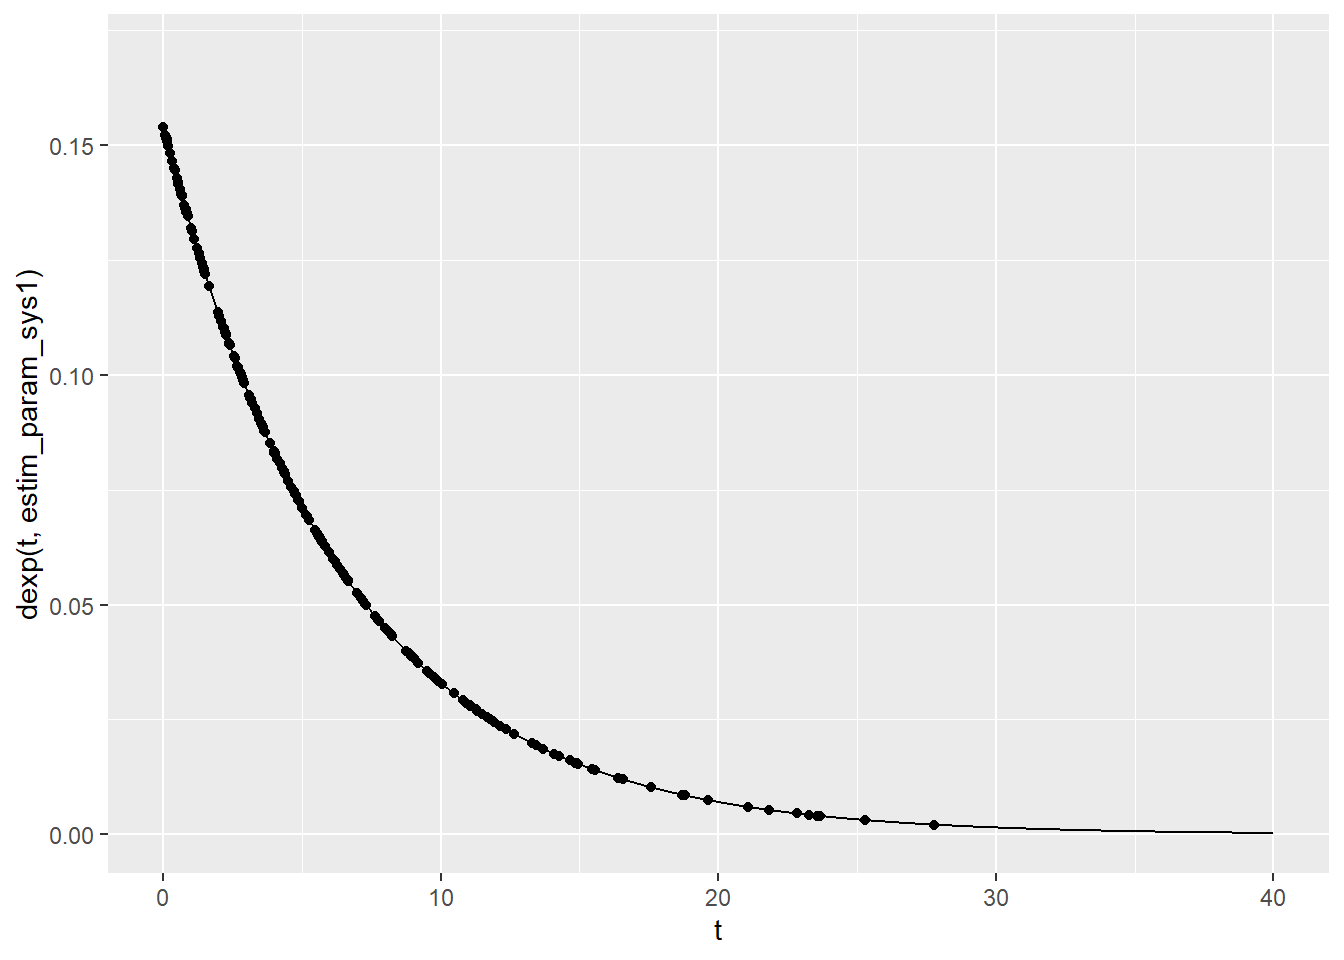
\includegraphics{exe6_files/figure-latex/unnamed-chunk-8-1.pdf}

On trouve une droite de régression. On peut chercher les paramètres de
la régression linéaire pour déterminer les paramètres de la loi
exponentielle.

\begin{Shaded}
\begin{Highlighting}[]
\FunctionTok{lm}\NormalTok{(}\SpecialCharTok{{-}}\FunctionTok{log}\NormalTok{(}\DecValTok{1}\SpecialCharTok{{-}}\NormalTok{i}\SpecialCharTok{/}\NormalTok{(n}\SpecialCharTok{+}\DecValTok{1}\NormalTok{)) }\SpecialCharTok{\textasciitilde{}} \FunctionTok{sort}\NormalTok{(xi)) }\SpecialCharTok{\%\textgreater{}\%} \FunctionTok{summary}\NormalTok{()}
\end{Highlighting}
\end{Shaded}

\begin{verbatim}
## 
## Call:
## lm(formula = -log(1 - i/(n + 1)) ~ sort(xi))
## 
## Residuals:
##      Min       1Q   Median       3Q      Max 
## -0.20628 -0.08132  0.01726  0.03967  0.92745 
## 
## Coefficients:
##             Estimate Std. Error t value Pr(>|t|)    
## (Intercept)  0.03121    0.01259    2.48    0.014 *  
## sort(xi)     5.61157    0.05258  106.72   <2e-16 ***
## ---
## Signif. codes:  0 '***' 0.001 '**' 0.01 '*' 0.05 '.' 0.1 ' ' 1
## 
## Residual standard error: 0.1251 on 198 degrees of freedom
## Multiple R-squared:  0.9829, Adjusted R-squared:  0.9828 
## F-statistic: 1.139e+04 on 1 and 198 DF,  p-value: < 2.2e-16
\end{verbatim}

On a \(R^2 = 0.9828\), et \(p_{value}=2.2 \times 10^{-16}\), ce qui nous
conforte dans l'adéquation des durées inter-pannes à une loi
exponentielle.

On a donc une estimation \(\lambda_{gph}=5.61157\).

On peut aussi chercher une estimation par méthode des moments :

\begin{Shaded}
\begin{Highlighting}[]
\DecValTok{1}\SpecialCharTok{/}\FunctionTok{mean}\NormalTok{(xi)}
\end{Highlighting}
\end{Shaded}

\begin{verbatim}
## [1] 5.870253
\end{verbatim}

Dans ce cas on a : \(\lambda_{gph}=5.870253\).

Donc on peut sans problème conserver l'hypothèse selon laquelle les
\(x_i\) suivent une loi exponentielle.

On peut tracer la courbe de la proportion de MP :

\begin{Shaded}
\begin{Highlighting}[]
\FunctionTok{ggplot}\NormalTok{() }\SpecialCharTok{+}
    \FunctionTok{geom\_line}\NormalTok{(}\FunctionTok{aes}\NormalTok{(}\AttributeTok{x =}\NormalTok{ i, }\AttributeTok{y =} \FunctionTok{cumsum}\NormalTok{(df[,}\StringTok{"ui"}\NormalTok{])}\SpecialCharTok{/}\NormalTok{i)) }\SpecialCharTok{+} 
    \FunctionTok{labs}\NormalTok{(}\AttributeTok{x =} \StringTok{"Mesures"}\NormalTok{,}
         \AttributeTok{y =} \StringTok{"Proportion de MP"}\NormalTok{,}
         \AttributeTok{title =} \StringTok{"Évolution des MP"}\NormalTok{)}
\end{Highlighting}
\end{Shaded}

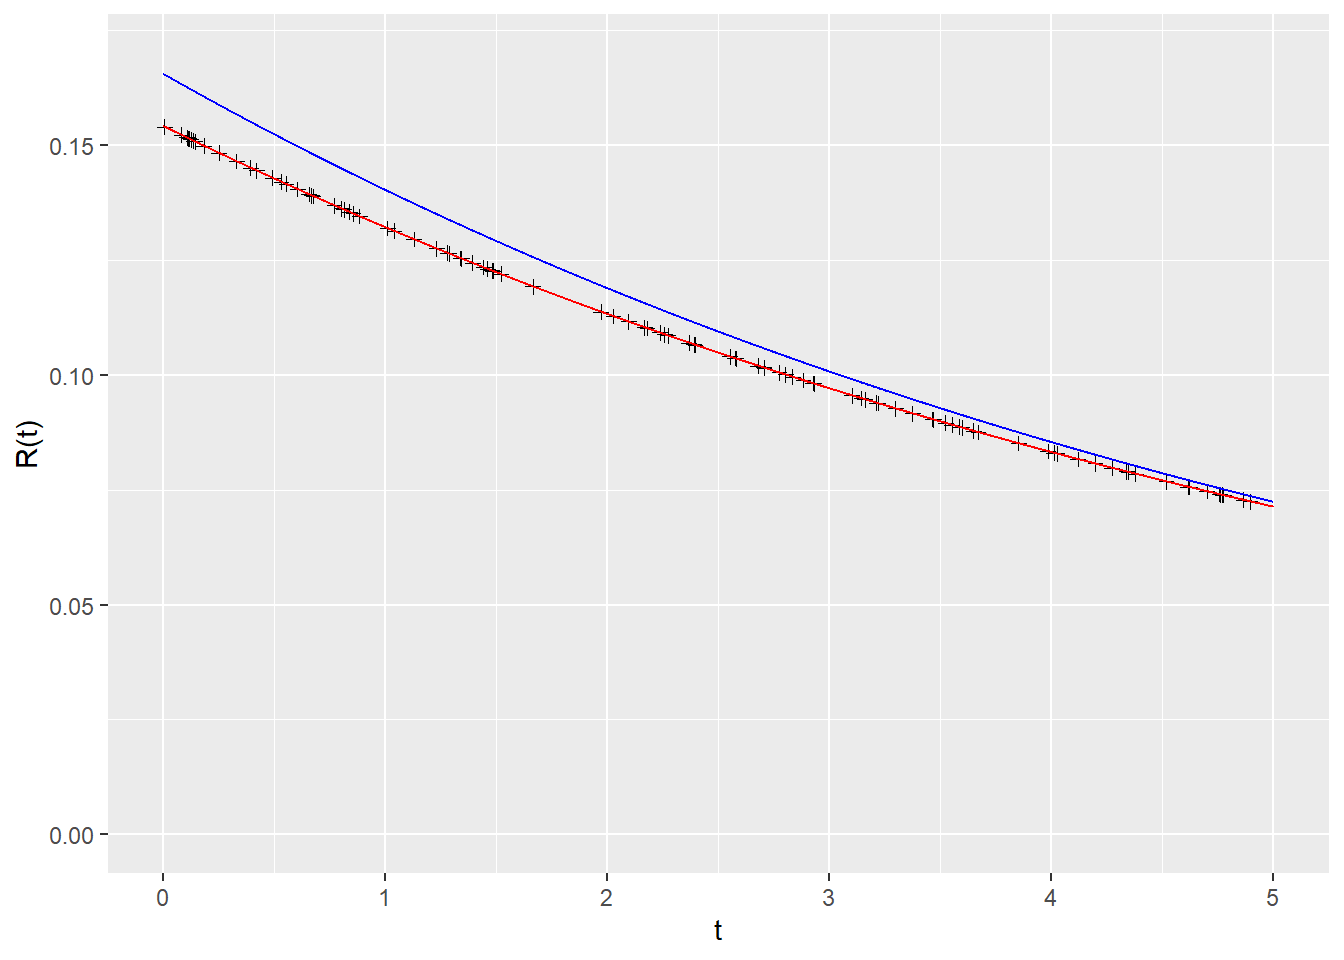
\includegraphics{exe6_files/figure-latex/unnamed-chunk-11-1.pdf}

Après quelques mesure, la proportion de MP semble se stabiliser vers
80\%. On effectue donc 80\% de maintenances préventives d'après les
données.

\subsection{Politique de maintenance}\label{politique-de-maintenance}

Après une maintenance, on suppose que la durée jusqu'à une MP est \(Y\)
et la durée jusqu'à une MC est \(Z\) avec \(Y\) et \(Z\) indépendants.

Dans ce cas la durée effective jusqu'à la prochaine maintenance est
\(W = min(Y,Z)\).

On suppose maintenant que \(Y \sim Exp(\mu)\) et
\(Z \sim Exp(\lambda)\).

Dans ce cas on cherche : \(P(W \leq w)\) :

\[
P(w \leq w) =
P(W \leq w | z \leq w)P(z \leq w) + \\
P(W \leq w | z > w)P(z > w)
\]

Avec :

\[
P(z \leq w) = 1-e^{-\lambda w} \\
P(z > w) = e^{-\lambda w} \\
P(W \leq w | z \leq w) = 1
\space \mbox{en effet quelque soit la valeur de y alors} \\
min(y,z)<w \mbox{ si } z \leq w \\
P(W \leq w | z > w) = P(y \leq w | z > w) = 1-e^{-\mu w}
\]

Dans ce cas :

\[
P(W \leq w) = (1 - e^{-\lambda w}) + (1- e^{-\mu w})
e^{-\lambda w}\\
= 1 - e^{-(\mu + \lambda) w}
\]

Donc \(W \sim Exp(\mu + \lambda)\) d'espérance \(\frac{1}{\mu+\lambda}\)

On cherche ensuite la probabilité \(\pi\) que la prochaine maintenance
soit une MP :

\[
\pi = P(y<z) = \int_{z \in \Omega_Z} F_Y(z)f_Z(z)dz\\ =
\int_{z \in \Omega_Z}(1-e^{-\mu z})\lambda e^{-\lambda z}dz
= \int_{z \in \Omega_Z} \lambda e^{-\lambda z} - 
\lambda e^{-\lambda z}e^{-\mu z} \\ =
\frac{\lambda}{\lambda} - \frac{\lambda}{\lambda + \mu} = 
1 - \frac{\lambda}{\lambda + \mu} = \frac{\mu}{\lambda + \mu}
\]

Dans notre jeu de données, la durée moyenne inter-pannes observée est de
:

\begin{Shaded}
\begin{Highlighting}[]
\FunctionTok{sprintf}\NormalTok{(}\StringTok{"Moyenne de durée inter{-}pannes : \%f"}\NormalTok{, }\FunctionTok{mean}\NormalTok{(xi))}
\end{Highlighting}
\end{Shaded}

\begin{verbatim}
## [1] "Moyenne de durée inter-pannes : 0.170350"
\end{verbatim}

Avec une proportion de MP de :

\begin{Shaded}
\begin{Highlighting}[]
\FunctionTok{sprintf}\NormalTok{(}\StringTok{"Proportion de MP : \%f"}\NormalTok{, }\FunctionTok{sum}\NormalTok{(df[,}\StringTok{"ui"}\NormalTok{])}\SpecialCharTok{/}\NormalTok{n)}
\end{Highlighting}
\end{Shaded}

\begin{verbatim}
## [1] "Proportion de MP : 0.815000"
\end{verbatim}

Dans ce cas on a : \(\pi = 0.815000\) et \(E[W] = 0.170350\), soit :

\[
\left\{
  \begin{array}{ll}
    \pi = \frac{\mu}{\lambda + \mu} \\
    E[W] = \frac{1}{\lambda + \mu}
  \end{array}
\right.
\]

Donc : \(\pi = \mu * E[W]\) donc \(\mu = \frac{\pi}{E[W]}\), et
\(\lambda = \frac{1}{E[W]}(1-E[W]\mu)\).

On peut alors estimer les paramètres :

\begin{Shaded}
\begin{Highlighting}[]
\FunctionTok{sprintf}\NormalTok{(}\StringTok{"mu = \%f"}\NormalTok{, }\FloatTok{0.815000}\SpecialCharTok{/}\FloatTok{0.170350}\NormalTok{)}
\end{Highlighting}
\end{Shaded}

\begin{verbatim}
## [1] "mu = 4.784268"
\end{verbatim}

\begin{Shaded}
\begin{Highlighting}[]
\FunctionTok{sprintf}\NormalTok{(}\StringTok{"lambda = \%f"}\NormalTok{, (}\DecValTok{1}\FloatTok{{-}0.170350}\SpecialCharTok{*}\FloatTok{0.815000}\NormalTok{)}\SpecialCharTok{/}\FloatTok{0.170350}\NormalTok{)}
\end{Highlighting}
\end{Shaded}

\begin{verbatim}
## [1] "lambda = 5.055267"
\end{verbatim}

Donc on a \(Y \sim Exp(4.784268)\) et \(Z \sim Exp(5.055267)\).

\subsection{\texorpdfstring{Indépendance entre \(U\) et
\(W\)}{Indépendance entre U et W}}\label{induxe9pendance-entre-u-et-w}

On va ensuite chercher à montrer que les variables aléatoires \(U\) et
\(W\) sont indépendante. On a :

\begin{itemize}
\tightlist
\item
  \(U\), le type de maintenance avec \(P(U=0)=1-\pi\) et \(P(U=1)=\pi\)
\item
  \(W\), la durée inter panne, de loi exponentielle de paramètre
  \(\mu+\lambda\).
\end{itemize}

Deux variables aléatoires \(A\) et \(B\) sont indépendantes si on a :
\(P(A=a \cap B=b)=P(A=a)P(B=b), \forall a\in \Omega_A \forall b \in \Omega_B\)

On cherche donc à montrer que par exemple \(P(W>w|U=1)=P(W>w)P(U=1)\).
Avec :

\begin{itemize}
\tightlist
\item
  \(P(W>w)=e^{-(\mu+\lambda)w}\)
\item
  \(P(U=1)=\pi\)
\end{itemize}

\[
P(W>w|U=1) = P(min(y,z)>w|y<z) = \int_{z\in \Omega_z}
P(y>w|Z=z,y<z)f_Z(z)dz
\]

\[
z < w, y < z \Rightarrow y <z < w \Rightarrow P(y>w|Z=z,y<z)=0 \\
z > w, y < z \Rightarrow P(y>w|Z=z,y<z)=
P(y\in[w,z])=R_Y(w)-R_Y(z)
\]

Donc :

\[
\begin{array}{ll}
P(W>w|U=1) & = \int_{z\in \Omega_z} P(y>w|Z=z,y<z)f_Z(z)dz \\
& = \int_{z}^{w}0f_Z(z)dz + \int_{w}^{+\infty}(R_Y(w)-R_Y(z))f_Z(z)dz \\
& = \int_{w}^{+\infty} \left( e^{-\mu w} - e^{-\mu z} \right) \lambda
e^{-\lambda z} dz \\
& = \lambda e^{-\mu w} \int_{w}^{+\infty}e^{-\lambda z}dz - 
\lambda \int_{w}^{+\infty} e^{-(\mu + \lambda) z}dz \\
& = e^{-\mu w} e^{-\lambda w} - e^{-(\mu + \lambda)w}\frac{\lambda}{\lambda+\mu}
= \frac{\mu}{\lambda + \mu}e^{-(\mu + \lambda)w} \\
& = P(U=1)P(W>w)
\end{array}
\]

Donc, la probabilité d'avoir une maintenance préventive est indépendante
de la valeur de \(W\).

\end{document}
